\subsection{Grådige algoritmer}
Når man arbejder med optimeringsproblemer, som omhandler minimering eller maksimering, dette kunne fx være at finde den længste eller korteste vej i en graf, kan man ofte bruge \emph{grådige algoritmer}.
En grådig algoritme vælger altid det \emph{lokalt optimale} valg og antager, at dette medfører en \emph{global optimal} løsning, altså den bedst mulige løsning. Det lokalt optimale valg findes ved at vælge den umiddelbart bedste løsning for hvert muligt trin.
I mange tilfælde vil dette lede til global optimering, men der kan også forekomme situationer, hvor algoritmen vil finde en suboptimal løsning. Ligegyldigt om algoritmen finder en optimal eller suboptimal løsning, kalder vi den en grådig algoritme. 
   
Grådige algoritmer bruges også i grafteori til fx at løse korteste eller længste vej-problemer. Her vælger algoritmen den lokalt optimale vej fra startknuden til en naboknude. En grådig algoritme ser nu bort fra alle andre muligheder som ikke bruger denne knude.

\begin{figure}[H]
\centering
	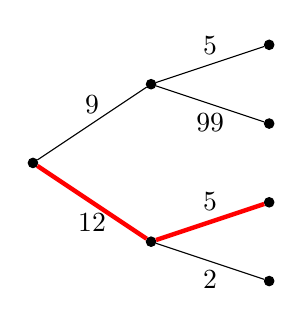
\begin{tikzpicture}

      \tikzset{enclosed/.style={draw, circle, inner sep=0pt, minimum size=.12cm, fill=black}}
% Vertices
      	\node[enclosed] (v1) at (0,2) {};
      	\node[enclosed] (v2) at (1.5,1) {};
    	\node[enclosed] (v3) at (1.5,3) {};
  	    \node[enclosed] (v4) at (3,0.5) {};
  	    \node[enclosed] (v5) at (3,1.5) {};
  	    \node[enclosed] (v6) at (3,3.5) {};
  	    \node[enclosed] (v7) at (3,2.5) {};    
%Edges
		\path (v1) edge[red, ultra thick] node[midway, below, black] {$12$} (v2);
		\path (v1) edge node[midway, above] {$9$} (v3);
		\path (v2) edge[red, ultra thick] node[midway, above, black] {$5$} (v5);
		\path (v2) edge node[midway, below] {$2$} (v4);
		\path (v3) edge node[midway, above] {$5$} (v6);
		\path (v3) edge node[midway, below] {$99$} (v7);


	\end{tikzpicture}
	\caption{Længste vej ifølge grådig algoritme.}
	\label{fig:greedy.eks}
\end{figure}

\autoref{fig:greedy.eks} et eksempel på en grådig algoritme, som har forsøgt at finde den længste mulige simple vej i en graf. Vi kan se, at algoritmen har valgt de lokalt optimale valg, men har ikke fundet den global optimale løsning. Det er tydeligt at se, at denne algoritme ikke er pålidelig nok til at løse sådanne problemer. Der findes dog nogle grådige algoritmer som er optimeret således de altid finder den globalt optimale løsning, så længe grafen overholde specifikke krav. Dette ser vi i \autoref{kap:dijkstras}

    

\begin{exmp}
Det danske møntsystem har seks forskellige mønter med værdier på $0.5,\ 1,\ 2,\ 5,\ 10$ og $20$ kroner. Systemet er optimeret således, at man kan lave byttepenge vha. en grådig algoritme. Man kan altid finde den optimale løsning ved at tage så mange af de mest værdifulde mønter først og derefter tage så mange som muligt af de næst mest værdifulde mønter. Man fortsætter denne proces, indtil man har den ønskede mængde byttepenge.
\begin{algorithm} [H]
\caption{Grådig algoritme til byttepenge}
\begin{algorithmic}[1]

\Procedure{Byttepenge($c_1,c_2,\dotsc,c_r$: værdien af mønter, hvor $c_1>c_2>\dotsb >c_r;n:$ et positivt heltal)}{}
\EndProcedure
\For{$i:=1$ \textbf{to} $r$}
    \State $d_i:=0$ ($d_i$ tæller mængden af mønter med værdi $c_i$)
    \While{$n \geq c_i$}
    	\State $d_i := d_i+1$ (Mængden af mønter med værdi $c_i$ øges med en.)
    	\State $n := n-c_i$
\EndWhile
\EndFor
\State ($d_i$ er mængden af mønter med værdi $c_i$ for $i=1,2,\dotsc,r$)
\end{algorithmic}
\end{algorithm}
Denne algoritme vil altid vælge den optimale løsning i dette specifikke problem, der kan dog være problemer, hvis mønternes værdi ændrer sig. 
Vi forestiller os nu, at vi har et møntsystem med udelukkende tre mønter af værdi $25$, $10$ og $1$. Der opstilles her et problem, hvor vi vil have $30$ kroner i byttepenge. Denne algoritme vil nu få en løsning, som bruger én mønt af værdi $25$ og fem mønter af værdi $1$. Dette er en suboptimal løsning, da man kunne have brugt tre mønter af værdi $10$.
Dette viser, at grådige algoritmer ikke altid finder den optimale løsning.
\end{exmp}

